\pagestyle{fancy}
\fancyhf{}
\fancyhead[LE, RO]{}
\fancyhead[LO]{1993г выпуск 5}
\fancyhead[RE]{1993г выпуск 5}
\fancyhead[CE]{\thepage}
\fancyhead[CO]{\thepage}
\fancyfoot[R]{}
\fancyfoot[L]{}
\fancyfoot[C]{}
\setcounter{page}{10}
\setcounter{footnote}{2}
\twocolumn
Cаша), т.е. все пары, в которых день недели содинён сдежурным на этот день:

\textit{(день недели, дежурный на этот день)}

Или абстрактного: пары вида 
\[(x,f(x)).\]

Только выбор этих пар и существенен для задания функции.

После этого примера вам, быть может, не покажется неожиданныс, такое опреденение: \textit{графиком функции $f$ называется множество всех пар\footnote{Всюду в этой статьеимеются ввиду "упорядоченные пары". Пара (1, 2) отличается от пары (2, 1). Первый и второй элементы пары могут совпадать: (1, 1) или (2, 2) - тоже пары.
}}
\[(x, y),\]
\textit{что: 1) первый элемент пары $x$ принадлежит области определения функции, 2) второй элемент пары $y = f(x)$.}

В нашем примере график функции $f$:

$Г_f$ = \{(пн, Петя), (вт, Коля), (ср, Саша), (чт, Володя), (пт, Петя), (cб, Коля), (вс, Саша)\}.
Для функций, заданных таблицей

\medskip
\begin{tabular}{|s|s|s|s|s|}
\hline
$x$ & $f_1$ & $f_2$ & $f_3$ & $f_4$ \\ \hline
A & A & B & A & B \\ \hline
B & A & B & B & A \\ \hline
\end{tabular}

в соответствии с данным определением получим графики 
$Г_1$ = \{(A, A), (B, A)\}, $Г_2$ = \{(A, B), (B, B)\}

$Г_2$ = \{(A, A), (B, B)\}, $Г_3$ = \{(A, B), (B, A)\}

Ясно, что для функций с конечной областью определения число элементов графика (т.е. число входящих в график пар) равно числу элементов области определения функции. Для функций с бесконечной областью определения все пары
\[(x,f(x))\]
выписать нельзя. Приходится описывать эти пары при помощи их свойств.

Например, для функции 
\[y = f(x) =\sqrt{1-x^2}\]
график состоит из всевозможных парчисел вида 
\[(x, \sqrt{1-x^2}),\]
т.е из всех пар $(x, y)$, для которых выполненны два условия:
\[x^2 + y^2 = 1 и  y \geq 0\]

Это определение графика функции можно записать в виде
\[Г_f = \{(x, y)| x^2 + y^2 = 1, y \geq 0\}\]

Самое общее определение можно записать в виде такой формулы\footnote{Мы воспользуемся стандартным обозначением, принятым в теории множеств. Запись $\{x| A(x)\}$ обозначает множество всех объектов $x$, удовлетворяющих условию $A(x)$. Например, $\{x| x^2 = 1\}$ - множество всех $x$, для которых $X^2 = 1$, т.е. множество из двух чисел: $\{+1, -1\}$.}:
\[Г_f = \{(x, y)| y^2 = f(x)\}.\]

Определив график функции, как множество пар, каждая из которых состоит из значения аргумента и значения функции, соответствующего этому значению аргумента, мы освободили понятие графика от всего случайного. В этом абстрактном понимании к каждой функции имеется один-единственный график.

\newpage 
\onecolumn

\begin{wrapfigure}{r}{0.4\textwidth}
  \begin{center}
    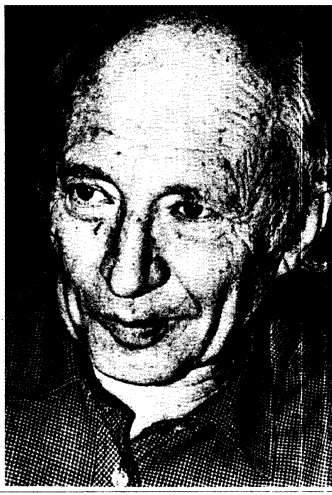
\includegraphics[scale=0.6]{photo.png}
  \end{center}
\end{wrapfigure}

\textit{\textbf{Поздравляем!}}
\\2 сентября 1933 года исполнилось 80 лет $\textit{Израилю Моисеевичу Гельфанду}$, академику РАН, профессору МГУ, почётному члену многих зарубежных академий. Один из крупнейших современных математиков, определивших развитие функционального анализа, автор многих работа по теоритической и прикладной математике и биологии на протяжении многих лет - начиная с 30-х годов - $\textit{И.М.Гельфанд}$ много сил вкладывает в воспитание молодых математиков, читает лекции для школьников, участвует в проведении московских олимпиад. В 60-е годы он был одним из основных организаторов и преподователей 2-й школы - одной из лучший матеематических школ в Москве.